\section{Model statyczny obiektu}
Przyjęty został następujący punkt pracy:
\begin{itemize}
	\item $x_{1_0} = 5,50677$
	\item $x_{2_0} = 0,132906$
	\item $x_{3_0} = 0,0019752$
	\item $x_{4_0} = 49,3818$
	\item $u_0 = 0,016783$
	\item $y_0 = 25000,911$
	\item $d_0 = 6,0$
\end{itemize}
Zakres dopuszczalnych sterowań został przyjęty jako $ u \in (0.0016783; 0.067132)$Z tego punktu wykonano serię skoków co $\Delta u = 0,0034$ i po każdym z nich odczekiwano 150 iteracji. Wyniki przedstawione zostały na rysunku \ref{fig:statyka-odpowiedzi}.
\begin{figure}[!h]
	\centering 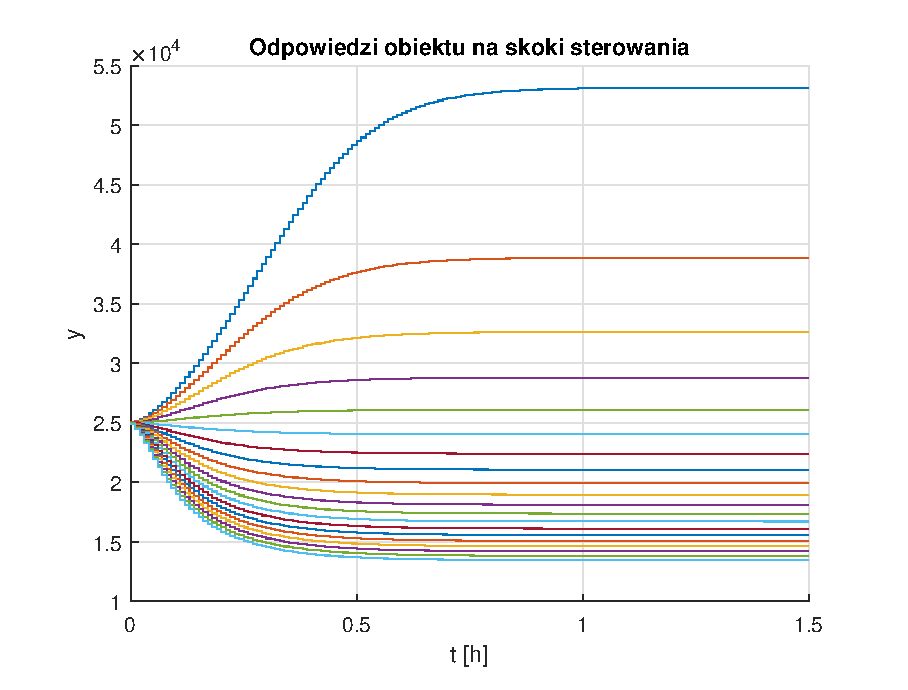
\includegraphics[width=0.8\linewidth]{statyka-odpowiedzi.eps}
	\caption{Odpowiedzi obiektu na skoki sterowania}
	\label{fig:statyka-odpowiedzi}
\end{figure}
Wartości z końca symulacji zostały zapisane do charakterystyki statycznej przedstawionej na rysunku \ref{fig:statyka-charakterystyka}.
\begin{figure}[!h]
	\centering \includegraphics[width=0.8\linewidth]{statyka-charakterystyka.eps}
	\caption{Charakterystyka statyczna obiektu}
	\label{fig:statyka-charakterystyka}
\end{figure}
Do modelowania charakterystyki użyto modelu Takagi-Sugeno o~czterech funkcjach przynależności przedstawionych na rysunku \ref{fig:mf}.
\begin{figure}[!h]
	\centering 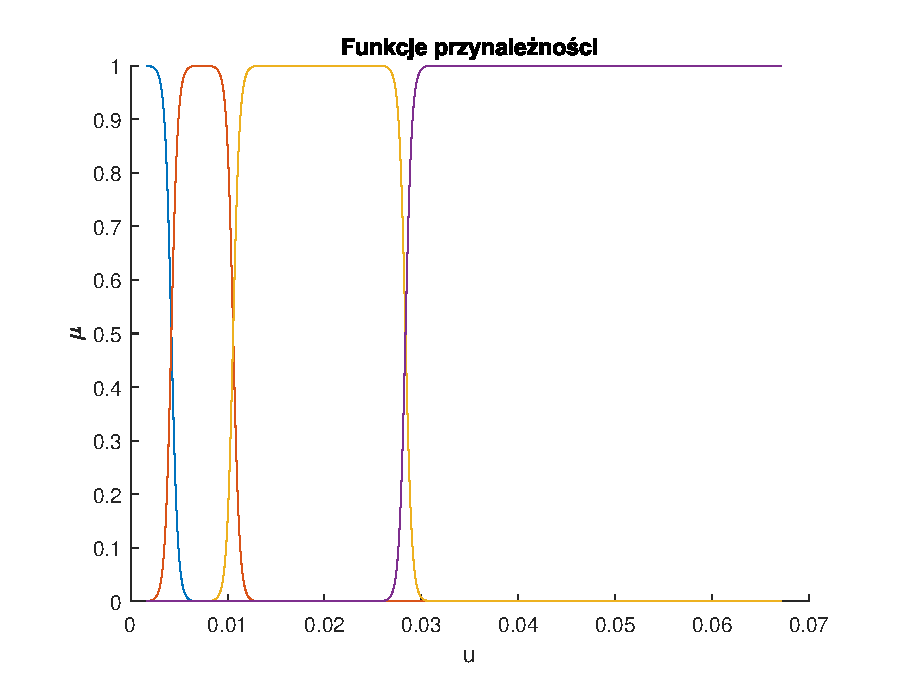
\includegraphics[width=0.8\linewidth]{mf.eps}
	\caption{Funkcje przynależności dla modelu statycznego obiektu}
	\label{fig:mf}
\end{figure}
\\Do każdej z nich przyporządkowany został model liniowy postaci:
\begin{equation}
y_{s_k}(u) = a_k\cdot u + b_k \qquad \textrm{gdzie } k = 1, 2, 3, 4
\end{equation}
Modele liniowe $y_{f_k}(u)$ uzyskano rozwiązując zadanie najmniejszych kwadratów na pewnym zakresie charakterystyki statycznej, zwiększając stopniowo ten zakres dopóki błąd średniokwadratowy pomiędzy modelem liniowym, a danymi nie przekroczył wartości progowej. Następnie zakres był przesuwany dalej i proces był powtarzany aż do osiągnięcia końcowej wartości $u$. Modele te przedstawione zostały na rysunku \ref{fig:modele-liniowe}.
\begin{figure}[!h]
	\centering 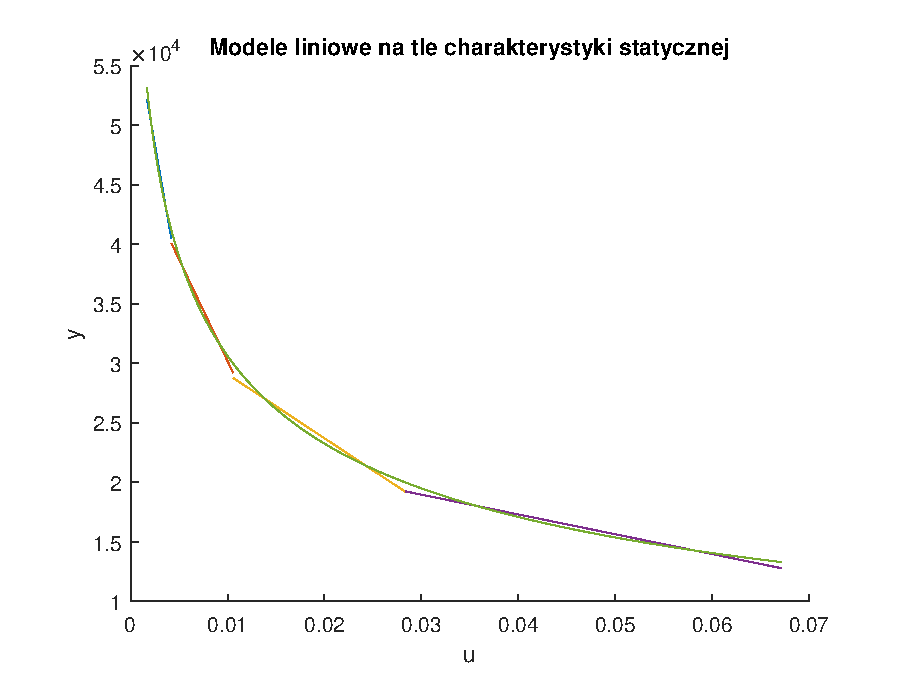
\includegraphics[width=0.8\linewidth]{modele-liniowe.eps}
	\caption{Funkcje przynależności dla modelu statycznego obiektu}
	\label{fig:modele-liniowe}
\end{figure}
Ostateczne wyjście modelu na tle charakterystyki statycznej przedstawiono na rysunku \ref{fig:statyka-model-rozmyty}.
\begin{figure}[!h]
	\centering 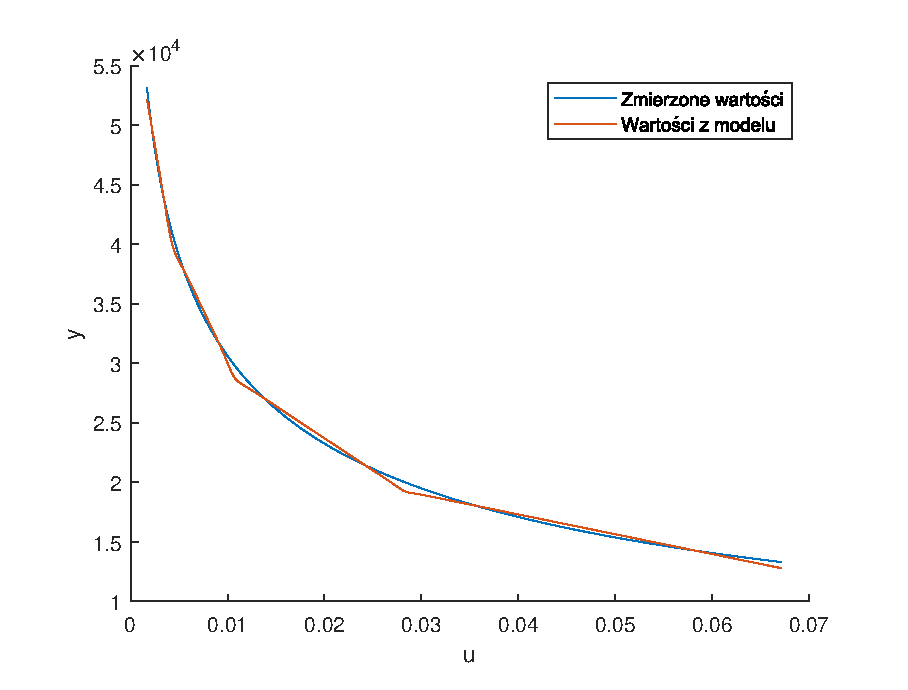
\includegraphics[width=0.8\linewidth]{statyka-model-rozmyty.eps}
	\caption{Wyjście rozmytego modelu statycznego}
	\label{fig:statyka-model-rozmyty}
\end{figure}
Błąd średniokwadratowy uzyskanego modelu wyniósł 1,29857e+05. Nie jest to bardzo dokładny model, jednakże bardziej skomplikowany model prowadziłby do zwiększenia nakładu obliczeniowego. Ponadto algorytmy regulacji całkują uchyb, przez co rozbieżności między modelem a obiektem będą kompensowane.